\section{\label{results}Results}

\subsection{Fundamental diagram in the original model}

In Fig~\ref{fundamental_diagram_flow}, we show the fundamental diagram (density vs. flow) for different corridor widths. We can distinguish the two typical branches of the fundamental diagram. In the free flow branch ($\rho < 5$), the flow increases linearly with the density since there are no collisions between pedestrians. This behavior holds for all the corridor's width. In the congested branch ($\rho > 5$), we have two different scenarios:


\begin{itemize}
\item i) In narrow corridors (say $w < 10$) we can see that the flow reduces as the density increases. This resembles the traditional behavior of the fundamental diagram reported in the literature. 
\item ii) In wide corridors (say $w > 15$) we see that the flow increases with density. This contradicts the typical behavior of the fundamental diagram.   
\end{itemize}

Since this discrepancy only appears in the congested branch, we can argue that the the friction force is playing a fundamental role in the flow reduction.  

In order to satisfy the fundamental diagram reported in the literature, It is necessary that the flow at the maximum density ($\rho_{max} = 9$) be less than the flow at $\rho = 5$. That is:  $J(\rho = 9) < J(\rho = 5)$. From the flow definition in Ec.~\ref{ec-flow} we can derive

\begin{align*} 
v(\rho_{max}) &< \frac{5v_d}{\rho_{max}} \\
v(\rho_{max}) &< \frac{5}{9} v_d
\end{align*}


As our desired velocity is fixed $v_d = 1$~m/s, we conclude that the speed at the maximum density has to be bounded by $v(\rho_{max}) \lesssim 	0.5$~m/s in order to satisfy the qualitative behavior of the fundamental diagram reported in the literature.\\

The above reasoning is consistent with the speed-density results shown in Fig.~\ref{fundamental_diagram_flow}. Notice that the speed values in $\rho_{max} = 9$ is higher than $v=0.5$~m/s for $w=15$~m and $w=22$~m. Whereas the speed value for $\rho_{max}$ is lower than $v=0.5$~m/s for narrow corridors ($w<15$)\\

\begin{figure}[htbp!]
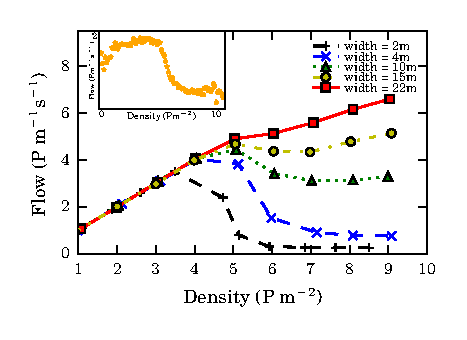
\includegraphics[width=\columnwidth]
{plots/flow-density_vd1_multiple_widths.eps}
\caption{\label{fundamental_diagram_flow} Flow as a function of the density for different widths. Initially, 
pedestrians were randomly distributed along the corridor. The measurements were taken in the middle
of the corridor once the system reached the stationary state. The length of the corridor 
was 28~m in all cases with periodic boundary conditions in the x direction.}
\end{figure}


\begin{figure}[htbp!]
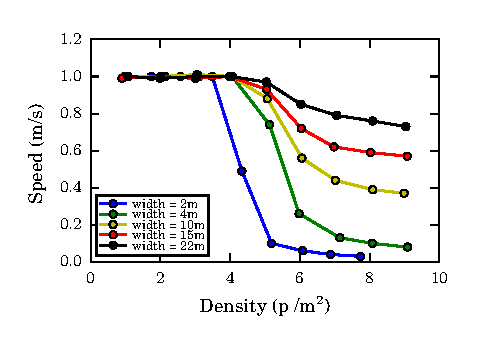
\includegraphics[width=\columnwidth]
{plots/speed-density_vd1_multiple_widths.eps}
\caption{\label{fundamental_diagram_speed} Speed as a function of the density for different widths. Initially, 
pedestrians were randomly distributed along the corridor. The measurements were taken in the middle
of the corridor once the system reached the stationary state. The length of the corridor 
was 28~m in all cases with periodic boundary conditions in the x direction.}
\end{figure}

\subsection{Speed profile}

In Fig.~\ref{speed-profile-w22} we show the speed profile (speed vs. y-position) of the pedestrians in the  corridor. When the density is low, pedestrians achieve the desired velocity ($v=v_d=1$~m/s), leading to a cruising velocity profile for every position in the corridor. For higher densities, the speed profile shifts to a parabola-like shape. Pedestrians near near the walls are the one with the lower speed. The speed increases when moving away from the wall until it reaches the maximum in the middle of the corridor. This behavior suggests that the friction that the wall exerts on pedestrians, is playing a fundamental role in the speed profile. We did some simulations removing the walls and adding periodic boundary conditions in the y-coordinate. This yield to constant-cruising speed profiles for all the densities, confirming that the walls are a necessary condition in order to produce a parabola-shaped speed profile.\\

%The pedestrian-wall friction es mayor que la friccion entree peatones porque la formula es asi...


\begin{figure}[htbp!]
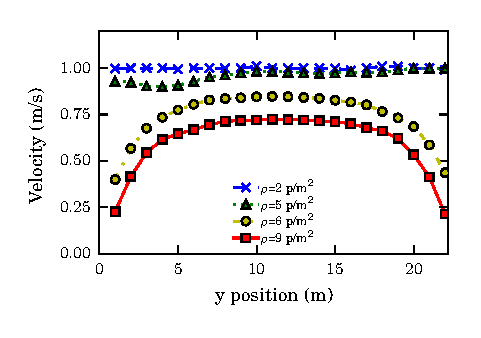
\includegraphics[width=\columnwidth]
{plots/v(y)_width22_k24.eps}
\caption{\label{speed-profile-w22} Speed profile (speed vs y-position) for different densities. The desired velocity was $v_d = 1$~m/s. The measurements were taken in $x=14$~m once the system reached the stationary state. The length of the corridor was 28~m in all cases with periodic boundary conditions in the x direction.  }
\end{figure}

\subsection{Friction modification}


\begin{figure}[htbp!]
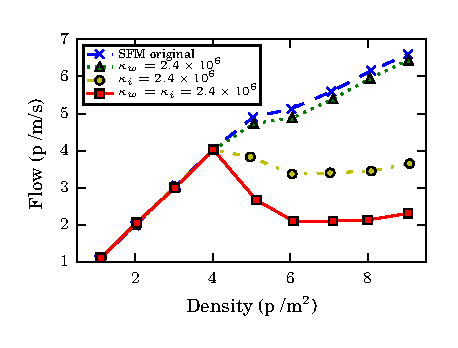
\includegraphics[width=\columnwidth]
{plots/flow-density_pasillo22m_fgmodified_multi.eps}
\caption{\label{fgmodified-w22} }
\end{figure}

